\subsection{Ajuste del modelo}\label{s:ajustes}

\begin{figure}[h!]
    \centering
    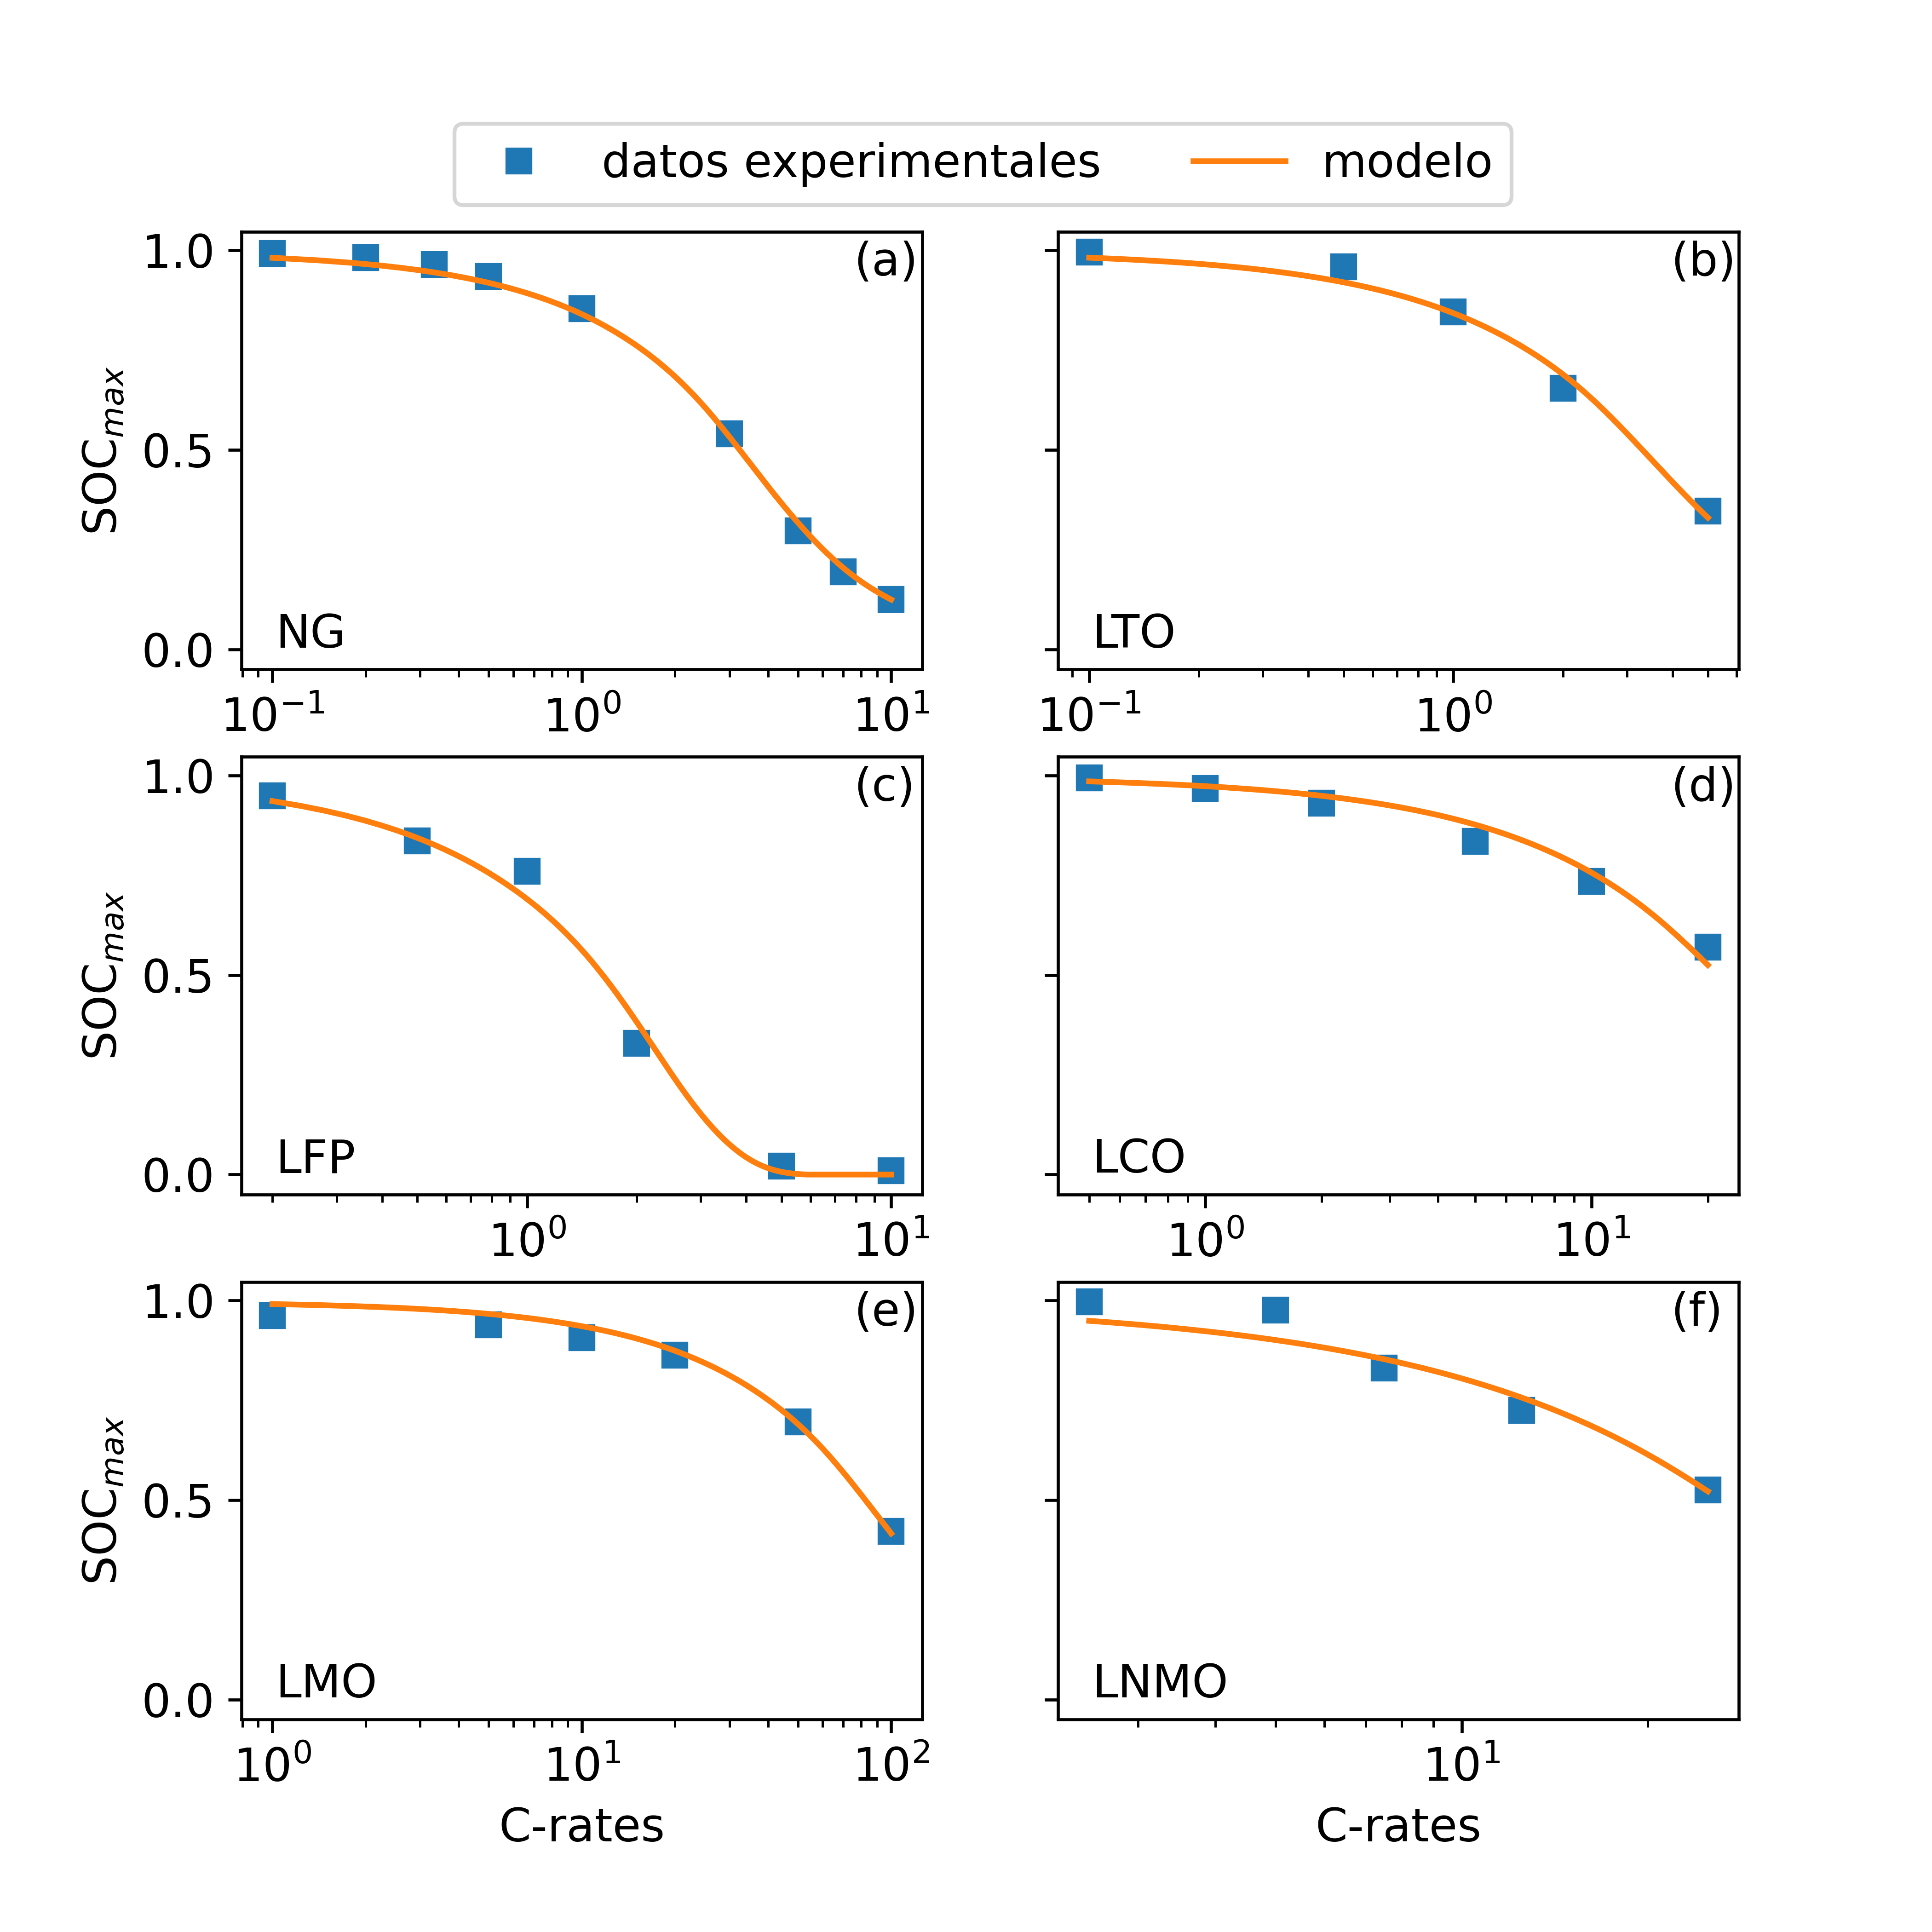
\includegraphics[width=0.7\textwidth]{FastCharging/un/resultados/ajuste/ajustes.png}
    \caption{Ajuste del modelo a los datos SOC$_{\max}$ \textit{versus} C-rate
    para los distintos materiales de electrodos considerados: (a) NG 
    \cite{mancini2022}, (b) LTO \cite{he2012}, (c) LFP \cite{lei2015}, 
    (d) LCO \cite{wang2019high}, (e) LMO \cite{bak2011}, (f) LNMO
    \cite{nishikawa2017}.}
    \label{fig:ajustes}
\end{figure}

En la Figura \ref{fig:ajustes} se muestran los datos experimentales y los 
ajustes del modelo para el SOC$_{\max}$ alcanzado al potencial de cortes 
\textit{versus} la C-rate para los resultados de la Figura \ref{fig:preproc}
y otros materiales de uso común en lso electrodos de las baterías de ion-litio.
Puede observarse una buena concordancia en general entre el modelo y los 
experimentos. Esto también puede observarse en la Figura \ref{fig:pred_vs_exp},
donde se muestran los valores predichos para SOC$_{\max}$ en función de los
experimentales, junto con el coeficiente de determinación de cada ajuste.

\begin{figure}[h!]
    \centering
    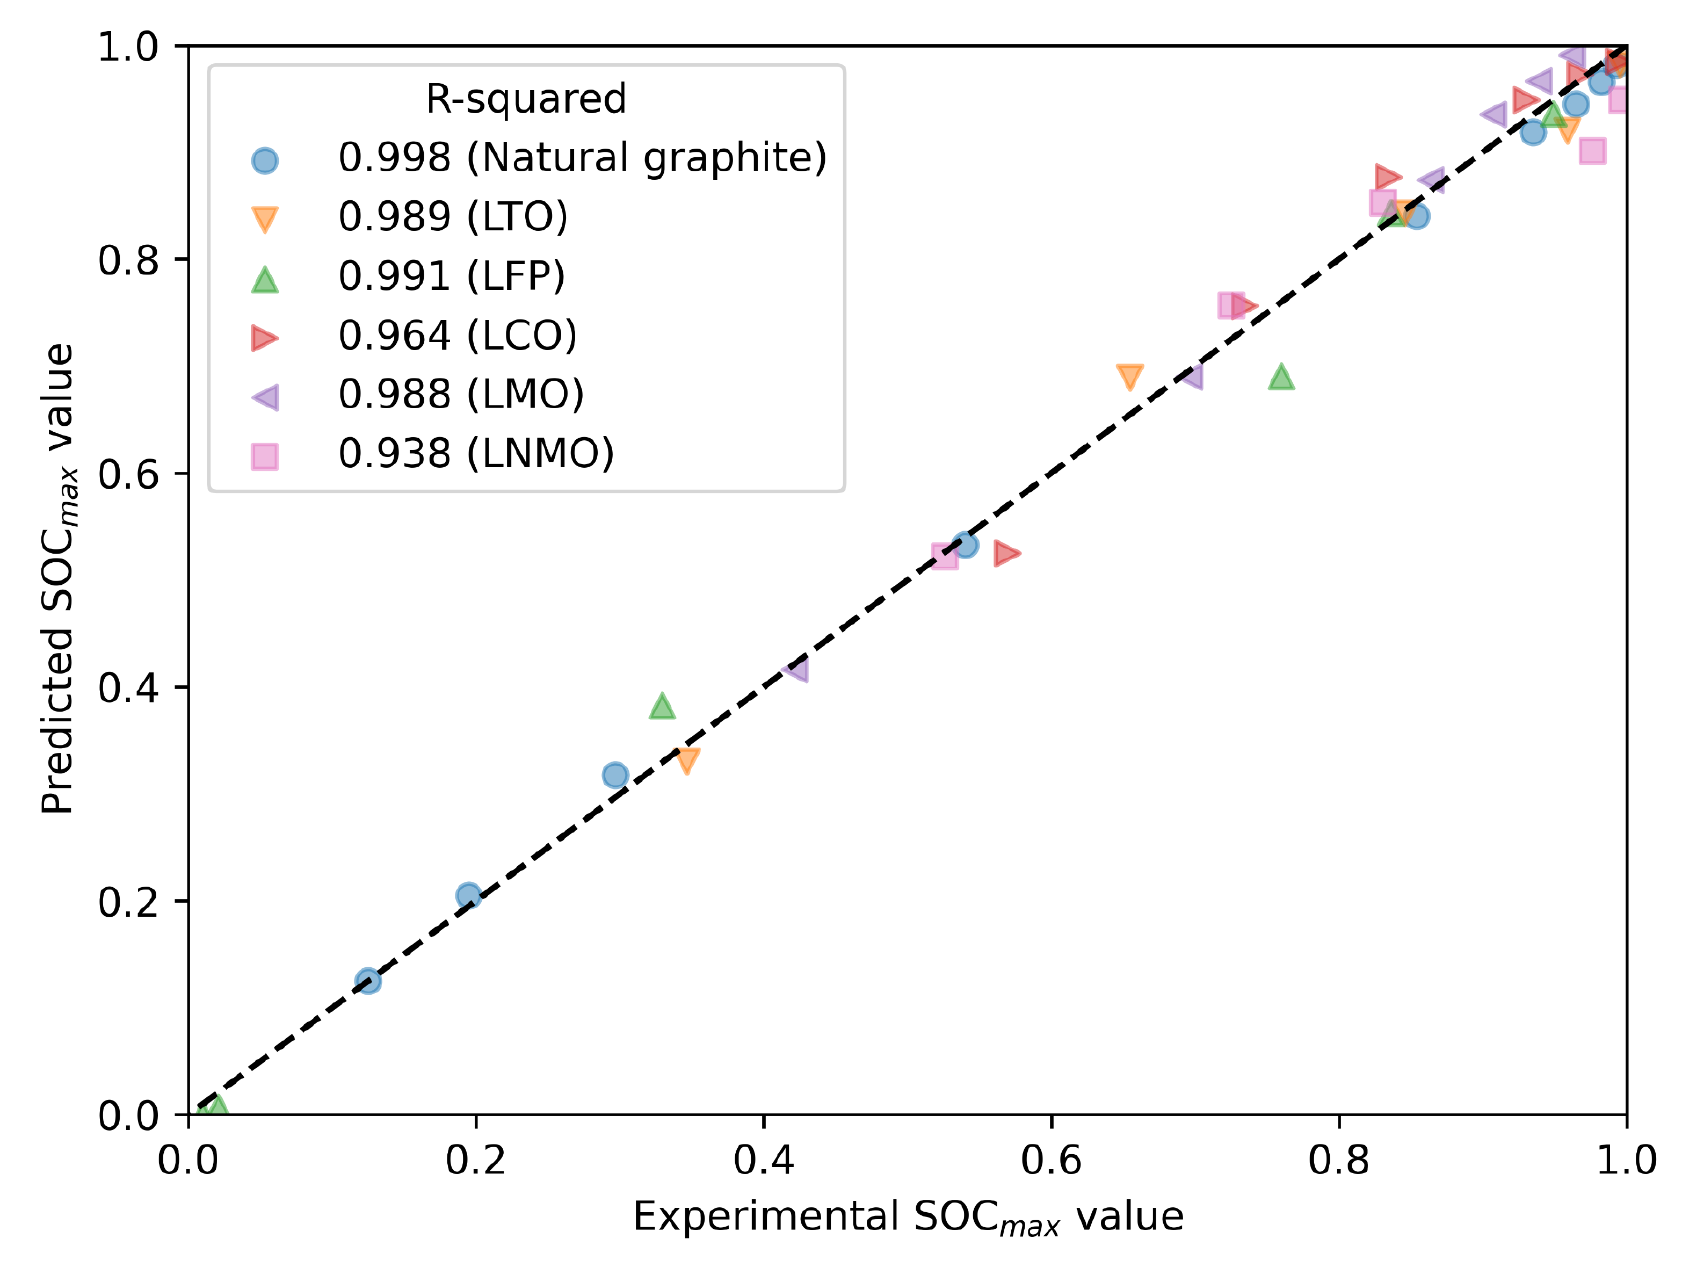
\includegraphics[width=0.7\textwidth]{FastCharging/un/resultados/ajuste/pred_vs_exp.png}
    \caption{Predicciones del SOC$_{\max}$ \textit{versus} valores 
    experimentales, junto al coeficiente de determinación de cada sistema $R^2$.}
    \label{fig:pred_vs_exp}
\end{figure}

El trabajo de Mancini \textit{et al} \cite{mancini2022} aportó nuevos 
conocimientos sobre el efecto de esferoidización en las características de las
partículas de grafito natural (NG) y su impacto en el comportamiento 
electroquímico. Como puede verse en la Figure \ref{fig:ajustes}a. En este caso, 
el rango de C-rates reportadas cubre una amplia región del SOC$_{\max}$, desde un 
material totalmente cargado hasta uno casi totalmente descargado. Esto no es lo 
habitual, ya que en la mayoría de los experimentos sólo se reportan curvas con un 
buen rendimiento (alta capacidad), lo que limita los ajustes realizados a una 
región concreta del diagrama. El coeficiente de difusión y la constante cinética 
obtenidos en el ajuste para este sistema son $1.23\times10^{-10}$ cm$^2$/s y 
$2.31\times10^{-7}$ cm/s, respectivamente. Para esto se consideró un tamaño
de partícula de $7.5 \mu$m y una geometría esférica. Este valor se corresponde
con la media de la distribución de tamaños, que es reportada junto a los 
cuartiles en el trabajo citado. Para los casos que siguen, en los que no se
tiene información precisa de la distribución de tamaños, se considera el punto
medio del rango reportado para el tamaño de las partículas y utiliza para 
definir el parámetro $d$ en el modelo.

Los ánodos de Li$_4$Ti$_5$O$_{12}$ (LTO) presentan características excelentes
de seguridad y una capacidad teórica de 175 mAhg$^{-1}$. He \textit{et al} 
\cite{he2012} sintetizaron nanopartículas cristalinas y esféricas de LTO a 
diferentes proporciones atómicas de Li/Ti, con un tamaño entre los 0.5 $\mu$m 
y los 3 $\mu$m. Se asume entonces un valor de $d=1.75 \mu$m y se utilizan los
datos de la proporción usual del LTO para ajustar el modelo, teniéndose como 
resultado un valor de $D$ de $6.58\times10^{-12}$ cm$^2$/s. El valor experimental 
de $D$ reportado por He \textit{et al} para esta proporción atómica fue de
$5.12\times10^{-12}$ cm$^2$/s. Con respecto al valor de $k^0$, se obtuvo 
$8.11\times10^{-8}$ cm/s. Comparar este valor con el experimental no es tan 
directo, ya que lo que reportan es la densidad de corriente de intercambio, 
$i^0 = 2.7\times10^{-4}$ mA/cm$^2$. Utilizando la ecuación \ref{eq:bv} de 
Butler-Volmer se tiene una relación entre $k^0$ e $i^0$ dada por
\begin{equation}\label{eq:i0k0}
    i^0 = F \frac{\rho}{M_r} k^0 \left(x_s\right)^{\alpha} \left(1 - x_s\right)^{1-\alpha},
\end{equation}
donde las definiciones de los parámetros están dadas en la Tabla \ref{t:params}.
Asumiendo un valor de 0.5 para el coeficiente de transferencia $\alpha$, un 
SOC de 0.5 y utilizando los valores del precursor LTO para $M_r = 459.1$ g/mol y
$\rho = 3.48$ g/cm$^3$ \cite{osti_1284125} se obtiene un valor para $k^0$ de
$7.38\times10^{-10}$ cm/s, que presenta una discrepancia de dos ordenes de 
magnitud con respecto al ajustado en el modelo. Sin embargo, en la literatura
se encuentran valores de $i^0$ con una gran dispersión entre 
$i^0 = 1.1\times10^{-3}$ mA/cm$^2$ \cite{medina2015} y $i^0 = 0.5$ mA/cm$^2$ 
\cite{umirov2019} que darían valores de $k^0$ entre $3.00\times10^{-9}$ cm/s y 
$1.37\times10^{-6}$ cm/s, respectivamente. Por lo cual puede afirmarse que el 
valor estimado por el modelo es razonable, dada la simplicidad del mismo.

Otro sistema en el cual las C-rates a las que se midieron los perfiles 
galvanostáticos cubren un rango amplio de valores de SOC$_{\max}$, de 
completamente cargado a completamente descargado, es el de LiFePO$_4$ (LFP) de 
Lei \textit{et al} \cite{lei2015}, como puede verse en la Figura 
\ref{fig:ajustes}. En este trabajo consideraron sistemas LFP/nanotubos de 
carbono/grafeno (LFP-CNT-G) como materiales catódicos con una capacidad 
superior a velocidades de carga alta y un desempeño favorable en sucesivos 
ciclados a densidades de corriente relativamente altas, comparados con 
sistemas LFP-CNT y LFP-G. Para este caso seleccionado, obtuvieron coeficientes 
de difusión, a partir de la pendiente de un ajuste lineal a mediciones de 
espectroscopia de impedancia electroquímica (EIS), de $1.04\times10^{-12}$ 
cm$^2$/s, $1.738\times10^{-13}$ cm$^2$/s y $8.225\times10^{-13}$ cm$^2$/s, 
respectivamente para cada uno de los sistemas mencionados. Mientras que al
ajustar los datos experimentales del primer sistema mencionado, con un tamaño
de partícula de $0.35 \mu$m, se obtuvo un valor de $2.85\times10^{-13}$ cm$^2$/s
para este parámetro. Como puede observarse, se aprecia una discrepancia de un 
orden de magnitud pero dentro de los valores obtenidos en las otras síntesis.
El valor obtenido para $k^0$ utilizando la ecuación \ref{eq:i0k0} y el dato 
$i^0=5.127\times10^{-4}$ mA/cm$^2$ es $1.23\times10^{-9}$ cm/s, con un valor
de $M_r$ de $157.75$ g/mol y $\rho$ de $1.36$ g/cm$^3$ \cite{jin2018}.
En este caso se encuentra una correspondencia excelente con el valor ajustado
de $1.00\times10^{-9}$ cm/s.

Para el caso del LCO se obtuvo un valor de $D$ de $5.34\times10^{-9}$ cm$^2$/s y
un valor de $k^0$ de $1.00\times10^{-5}$ al ajustar los datos experimentales 
de Wang \textit{et al} \cite{wang2019high}, ya presentados en la Figura 
\ref{fig:preproc} y ahora en el formato en el cual son ajustados en la Figura 
\ref{fig:ajustes}d. En dicho trabajo sintetizaron partículas esféricas en el rango
de 5 a 40 $\mu$m y utilizaron una técnica de microelectrodo de una sola partícula,
la cual les permitió seleccionar partículas de 20 $\mu$m por lo que este fue el
valor utilizado para $d$. El recubrimiento de TiO$_2$ mejora la eficiencia 
coulómbica, el rendimiento de la sobrecarga, la \textit{rate capability} y la
estabilidad con los ciclos a alto voltaje. El valor ajustado para el coeficiente 
de difusión se encuentra en el rango de los presentados en este trabajo 
(10$^{-10}$--10$^{-8}$) en la ventana de potencial 4.0--4.4 V.

Bak \textit{et al} \cite{bak2011} sintetizaron nanopartículas híbridas de la 
espinela LiMn$_2$O$_4$ (LMO) con óxido de grafeno reducido de unos 0.01--0.04 
$\mu$m. Con la geometría esférica considerada y el tamaño característico de 
difusión de 0.025 $\mu$m se obtuvo un $D$ de $3.51\times10^{-14}$ cm$^2$/s y una
$k^0$ de $1.87\times10^{-8}$ cm/s. El ajuste se muestra en la Figura 
\ref{fig:ajustes}e.

Por último, en la Figura \ref{fig:ajustes}f, se tiene la fase espinela 
LiNi$_{0.5}$Mn$_{1.5}$O$_4$ (LNMO), que es un material prometedor para ser 
utilizado como cátodo debido a su voltaje alto de funcionamiento de 4.7 V vs. 
Li$^+$/Li. En este caso, Nishikawa \textit{et al} \cite{nishikawa2017} también
utilizaron una técnica de medición de una sola partícula para este sistema con 
diámetros en el rango de 10 a 20 $\mu$m. En su trabajo estimaron el área 
superficial de la partícula seleccionada, asumiendo una forma esférica, de donde
se obtuvo un tamaño de partícula de 8 $\mu$m. Los valores ajustados para el
coeficiente de difusión y la constante cinética son $1.23\times10^{-9}$ cm$^2$/s 
y $1.23\times10^{-6}$ cm/s, respectivamente. Como se realizó en los casos del 
LTO y LFP, se obtuvo un valor de la $k^0$ al utilizar la densidad de corriente
de intercambio reportada por Nishikawa \textit{et al}, 0.2 mA/cm$^2$. Además,
se utilizó $M_r$ y $\rho$ de 182.7 g/mol y 2.3 g/cm$^3$, respectivamente, y se
obtuvo $k^0 = 3.29\times10^{-7}$, que sólo difiere en un orden de magnitud con 
el valor ajustado.

\begin{figure}[h!]
    \centering
    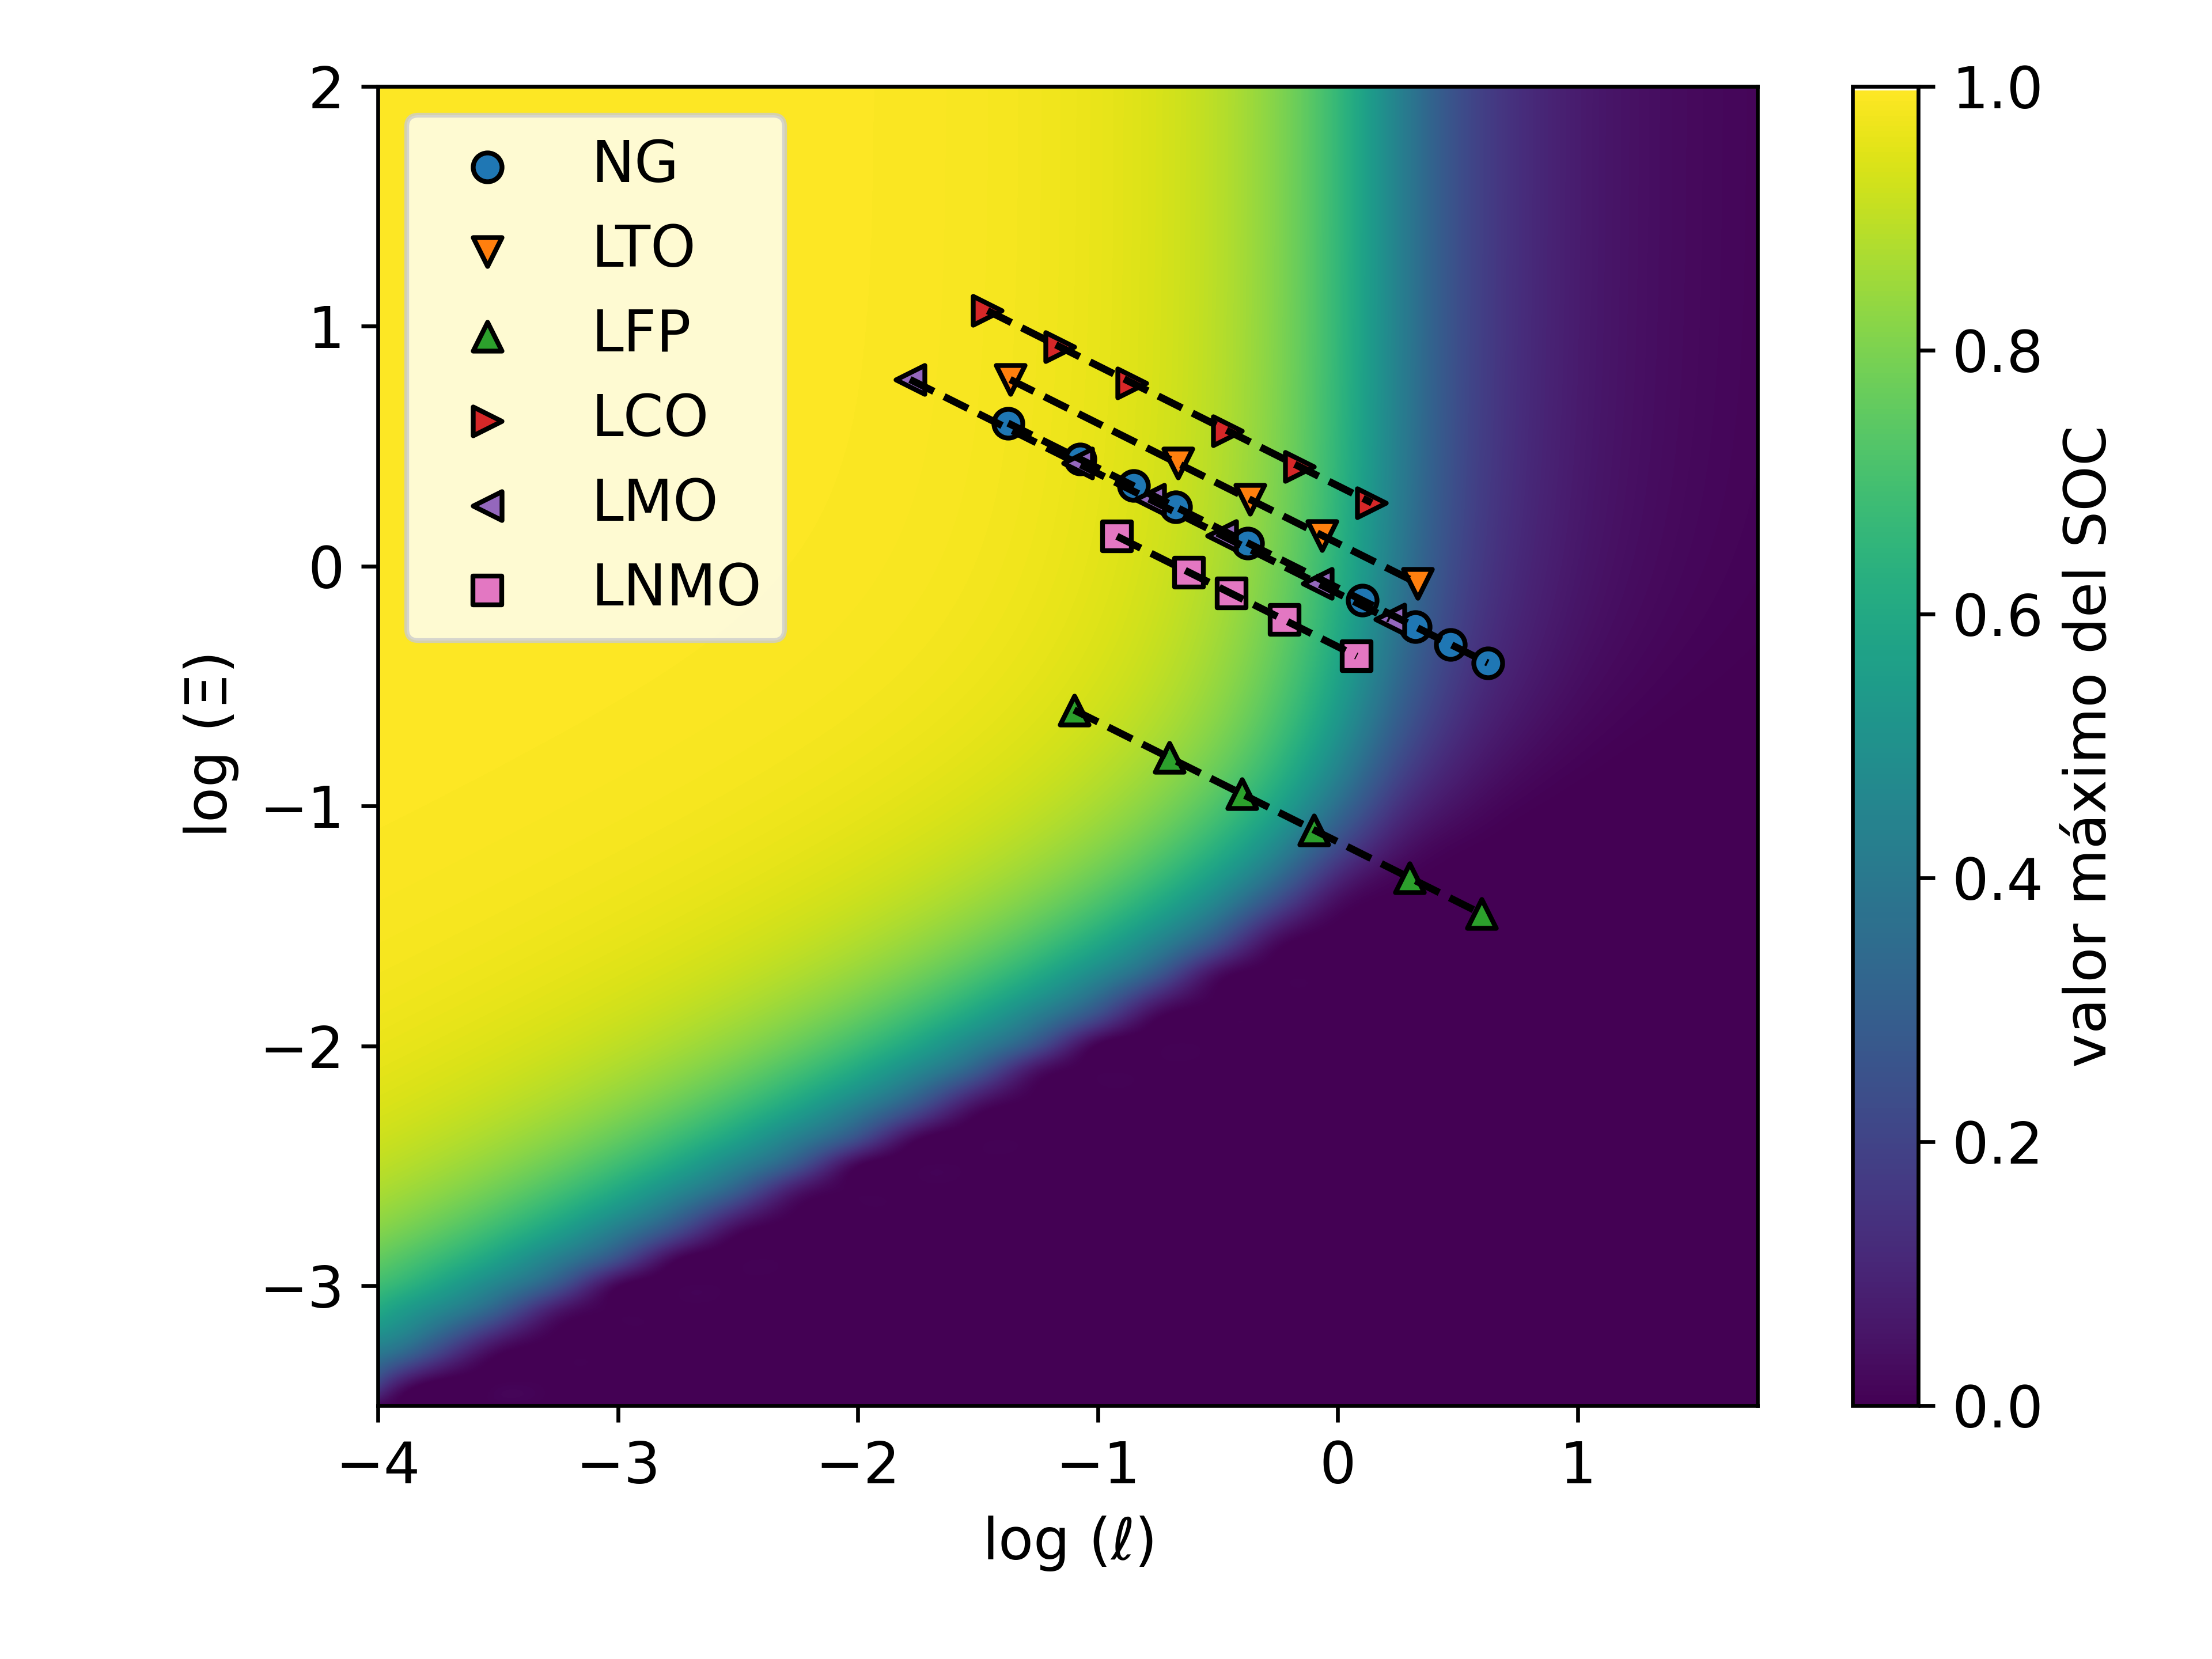
\includegraphics[width=0.7\textwidth]{FastCharging/un/resultados/ajuste/mapa.png}
    \caption{La región del diagrama en la que se encuentra cada experimento 
    \cite{mancini2022, he2012, lei2015, wang2019high, bak2011, nishikawa2017}
    luego del ajuste.}
    \label{fig:ajustes-mapa}
\end{figure}

También es ilustrativo presentar los ajustes realizados con el modelo 
heurístico en la superficie construida con las simulaciones galvanostáticas, 
como se muestra en la Figure \ref{fig:ajustes-mapa}, donde se tiene el valor
de SOC$_{\max}$ en el plano $\log(\Xi)$--$\log(\ell)$.

\begin{table}[h!]
    \centering
    \caption{Valores ajustados para $D$ y $k^0$ con su incerteza 
    correspondiente.} 
    \setlength\extrarowheight{2pt}\stackon{%
    \begin{tabular}{l c c}
        \toprule
        \textbf{Material del electrodo} & 
        \textbf{$D$ [cm$^2$/s]} &  
        \textbf{$k^0$ [cm/s]} \\
        \midrule
        Grafito natural \cite{mancini2022} & (1.233 $\pm$ 0.001)$\times10^{-10}$ & (2.31 $\pm$ 0.01)$\times10^{-7}$ \\
        LTO \cite{he2012} & (6.58 $\pm$ 0.06)$\times10^{-12}$ & (8.1 $\pm$ 0.7)$\times10^{-8}$ \\
        LFP \cite{lei2015} & (2.8 $\pm$ 0.1)$\times10^{-13}$ & (1.00 $\pm$ 0.03)$\times10^{-11}$ \\
        LCO \cite{wang2019high} & (5.3 $\pm$ 0.2)$\times10^{-9}$ & (1.0 $\pm$ 0.9)$\times10^{-5}$ \\
        LMO \cite{bak2011} & (3.51 $\pm$ 0.03)$\times10^{-14}$ & (1.9 $\pm$ 0.1)$\times10^{-8}$ \\
        LNMO \cite{nishikawa2017} & (1.2 $\pm$ 0.3)$\times10^{-9}$ & (1.2 $\pm$ 0.9)$\times10^{-6}$ \\
        \bottomrule
    \end{tabular}
    }{}
    \label{t:dk0}
\end{table}

Los parámetros obtenidos de los ajustes para los distintos materiales están
agrupados en la Tabla \ref{t:dk0} con su incerteza correspondiente. Las mismas
fueron calculadas usando la matriz de covarianza de los parámetros del modelo. 
Para ello se supone que la incerteza en C-rate es mucho menor que en 
SOC$_{\max}$ y que los parámetros del modelo dependen de estos valores, 
entonces dicha matriz está estrechamente relacionada a sus incertidumbres
\begin{equation}
    \sigma_{a_j, a_k}^2 = \sum_{i=0}^{N-1} \frac{\partial a_k}{\partial \text{SOC}_{\max,i}} \frac{\partial a_j}{\partial \text{SOC}_{\max,i}},
\end{equation}
donde en este caso $a_j$ y $a_k$ pueden ser $D$ y $k^0$. Las incertezas en 
estos parámetros están dadas en la diagonal de la matriz,
\begin{equation}
    \sigma_D^2 = \sum_{i=0}^{N-1} \left(\frac{\partial D}{\partial \text{SOC}_{\max,i}}\right)^2
\end{equation}
y
\begin{equation}
    \sigma_{k^0}^2 = \sum_{i=0}^{N-1} \left(\frac{\partial k^0}{\partial \text{SOC}_{\max,i}}\right)^2.
\end{equation}
Si tuviéramos una expresión analítica, i.e. si conociéramos la expresión 
explícita dada en la ecuación \ref{eq:socmax}, se podría calcular fácilmente
estos valores. Dado que este no es el caso, lo que se hace es resolverlo 
numéricamente aproximando la matriz de covarianza por la inversa de la matriz
Hessiana, que a su vez también es aproximada por el producto de la matriz
Jacobiana con su transpuesta \cite{bard1974}.
